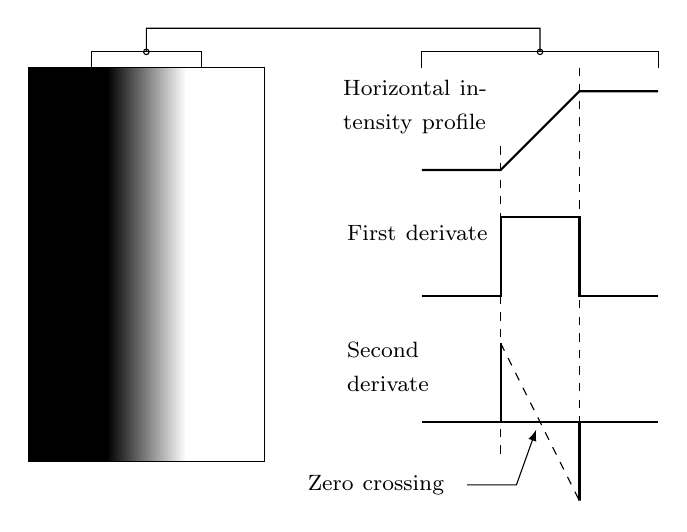
\begin{tikzpicture}
	\begin{scope}
		\fill (0,0) rectangle (1,5);
		\shade[shading angle=90, left color = black, right color = white] (1,0) rectangle (2,5);
		\fill[color=white] (2,0) rectangle (3,5);
		\draw (0,0) rectangle (3,5);
	\end{scope}
	\draw (0.8,5) -- ++(0,0.2) -- ++(1.4, 0) -- +(0,-0.2) ;
	\draw (5,5) -- ++(0,0.2) -- ++(3,0) -- +(0,-0.2);
	\draw[radius=1pt] (1.5,5.2) circle -- ++(0, 0.3) -- ++(5,0) -- ++(0,-0.3) circle;
	
	\begin{scope}[xshift=5cm]
		\begin{scope}[thick]
			\draw[yshift=3.7cm] (0,0) -- ++(1,0) -- ++(1,1) -- +(1,0);
			\draw[yshift=2.1cm] (0,0) -- ++(1,0) -- ++(0,1) -- ++(1,0) -- ++(0, -1) -- +(1,0);
			\draw[yshift=0.5cm] (0,0) -- ++(1,0) -- +(0,1) -- +(0,0) -- ++(1, 0) -- +(0,-1) -- +(0,0) -- +(1,0);
		\end{scope}
		\draw[dashed] (1,4) -- +(0,-4);
		\draw[dashed] (2,5) -- +(0,-5);
		\draw[yshift=0.5cm, dashed] (1,1) -- (2,-1);
		
		\node[text width=2cm] at (0,4.5) {\footnotesize Horizontal intensity profile};
		\node[text width=1.9cm] at (0,2.9) {\footnotesize First derivate};
		\node[text width=1.9cm] at (0,1.2) {\footnotesize Second derivate};
		\node[text width=1.9cm] (zc) at (-0.5,-0.3) {\footnotesize Zero crossing};
		\draw[-latex] (zc) -- ++(1.7, 0) -- +(0.25, 0.7);		
	\end{scope}		
\end{tikzpicture}